% !TEX program = xelatex
% Homework template

\documentclass[cn,12pt]{homework}
% en is for English language
% cn is for Chinese language

%----- text fonts -----
%\usepackage{newtxtext}
%\setmainfont{Times New Roman}

%----- math font -----
%\usepackage{newtxmath}
%\usepackage{mathptmx}
%\usepackage{mathpazo}

%----- custom theorem -----
\newtheorem{innercustomgeneric}{\customgenericname}
\providecommand{\customgenericname}{}
\newcommand{\newcustomtheorem}[2]{%
  \newenvironment{#1}[1]
  {%
   \renewcommand\customgenericname{#2}%
   \renewcommand\theinnercustomgeneric{##1}%
   \innercustomgeneric
  }
  {\endinnercustomgeneric}
}

\newcustomtheorem{ntheorem}{定理}
\newcustomtheorem{nlemma}{引理}

%----- list style -----
\setlist{nolistsep}

% differential operator
\newcommand{\dif}{\mathop{}\!\mathrm{d}}

% new command
\newcommand{\CC}{\ensuremath{\mathbb{C}}}
\newcommand{\RR}{\ensuremath{\mathbb{R}}}
\newcommand{\A}{\mathcal{A}}
\newcommand{\bA}{\boldsymbol{A}}
\newcommand{\ii}{\mathrm{i}\,}
\newcommand{\dx}[1][x]{\mathop{}\!\mathrm{d}#1}
\newcommand{\abs}[1]{\lvert#1\rvert}
\newcommand{\norm}[1]{\left\lVert#1\right\rVert}
\newcommand{\red}[1]{\textcolor{red}{#1}}

%----------------------------------------------------
%	HOMEWORK INFORMATION
%----------------------------------------------------

\header{\itshape XX 课程 -- 作业 \#1} % 页眉
\footer{\itshape 学生名字} % 页脚


\title{作业 \#1} % 作业名字

\date{日期: \today} % 日期

\institute{XX 大学 XX 学院} % 学院或学校

\courseinfo{课程: XX 课程 } % 课程信息

\studentinfo{姓名: \textit{学生名字} \quad 专业: \textit{专业名称} \quad 学号: 123002584} % 学生信息


\begin{document}

\maketitle

%----------------------------------------------------
%	作业内容
%----------------------------------------------------

%\section*{作业题目}

%------------------------------%

\begin{problem}
这里是一个问题.
\end{problem}

\begin{solution}
这里是问题的解答.
\end{solution}

%------------------------------%

\begin{problem}
这里是一个证明问题.
\end{problem}

\begin{proof}
这里是问题的证明.
\end{proof}

%------------------------------%

\begin{hframe}
这里定义了一个新的盒子环境 \verb|hframe|, 它是没有编号的.
使用者可以写问题, 或者答案, 或者其他任何内容.
\begin{enumerate}
  \item 第一项
  \item 第二项
  \item 第三项
\end{enumerate}
\end{hframe}


%------------------------------%

\section*{定理环境}

\begin{definition}\label{def:foo}
这是一个定义.
\end{definition}

\begin{proposition}\label{prop:foo}
这是一个命题.
\end{proposition}

\begin{lemma}[Lemma]\label{lmm:foo}
这是一个引理.
\end{lemma}

\begin{theorem}[Theorem]\label{thm:foo}
这是一个定理.
\end{theorem}
\begin{proof}
这是证明环境.
\end{proof}

\begin{corollary}\label{cor:foo}
这是一个推论.
\end{corollary}

\begin{proposition}[Proposition]
这是一个命题.
\end{proposition}

\begin{remark}\label{rem:remark}
这是一个 remark.
\end{remark}

\begin{example}
这是一个例子.
\end{example}

\begin{ntheorem}{A.1}
这是一个自定义的定理.
\end{ntheorem}


%----------------------------------------------------

\clearpage

\section*{表格}
这是一个表格示例, 如表~\ref{tab:foo}

\begin{table}[ht!]
\centering
% PLCR已经定义
\caption{表格名字}
\label{tab:foo}
\begin{tabularx}{0.9\textwidth}{P{1cm}CCCCCC}
\toprule
A & $N=3$ & $N=5$ & $N=7$ & $N=9$ & $N=11$ & $N=13$ \\
\midrule
B & 1.5789 & 1.3478 &1.0645&0.8780 &0.7222 &0.5942  \\
C &  1.0000 &1.0000 &1.0000 &1.0000 &1.0000 &1.0000  \\
D &7.2632 &14.3913 &21.0323 &27.3171 &30.9630 &34.0870  \\
\bottomrule
\end{tabularx}
\end{table}

%\begin{table}[ht!]
%\caption{表格名字}
%\label{tab:foo}
%\centering
%\begin{tabular}{lllllll}
%\toprule
%A & $N=3$ & $N=5$ & $N=7$ & $N=9$ & $N=11$ & $N=13$ \\
%\midrule
%B & 1.5789 & 1.3478 &1.0645&0.8780 &0.7222 &0.5942  \\
%C &  1.0000 &1.0000 &1.0000 &1.0000 &1.0000 &1.0000  \\
%D &7.2632 &14.3913 &21.0323 &27.3171 &30.9630 &34.0870  \\
%\bottomrule
%\end{tabular}
%\end{table}


\section*{图片}
这是一个插图示例, 如图~\ref{fig:image1}.

\begin{figure}[htp!]
\centering
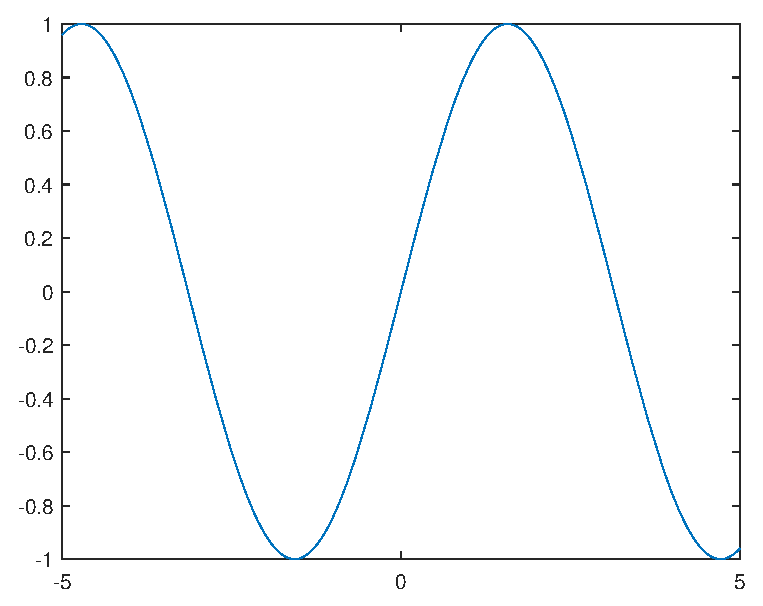
\includegraphics[width=0.48\textwidth]{image1}
\caption{函数 $y=\sin(x)$ 的图像}
\label{fig:sinx}
\end{figure}

这是一个两个图片并排放置的示例, 如图~\ref{fig:image1} 和 图~\ref{fig:image2}.

\begin{figure}[!htp]
\begin{minipage}[h]{0.48\linewidth}
\centering
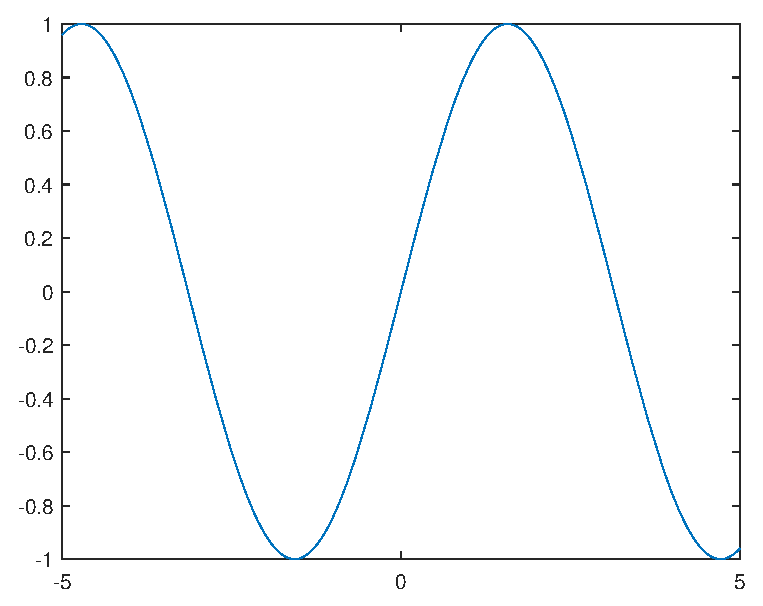
\includegraphics[width=0.9\textwidth]{image1}
\caption{图像一的描述}
\label{fig:image1}
\end{minipage}
\begin{minipage}[h]{0.48\linewidth}
\centering
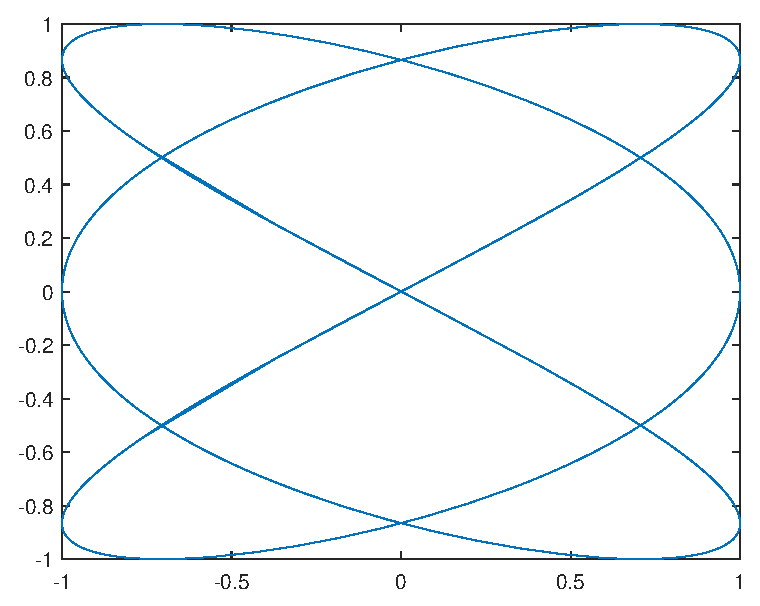
\includegraphics[width=0.9\textwidth]{image2}
\caption{图像二的描述}
\label{fig:image2}
\end{minipage}
\end{figure}


\clearpage
\section*{代码高亮}

这是 MATLAB 程序代码高亮环境.

% set code font
%basicstyle=\footnotesize\fontspec{Courier New}
%basicstyle=\footnotesize\fontspec{Consolas}

\begin{lstlisting}[style=matlab,basicstyle=\footnotesize\fontspec{Courier New},title={MATLAB code}]
% Euler method for the ODE model
% u'(x)=x^2+x-u, x in [0,1]
% Initial condition: u(0)=0.
clear all;  clf
h=0.1;
x=0:h:1;
N=length(x)-1;
u(1)=0;
fun=@(t,u) t.^2+t-u;   % RHS
for n=1:N
    u(n+1)=u(n)+h.*fun(x(n),u(n));
end
ue=-exp(-x)+x.^2-x+1;  % exact solution
plot(x,ue,'b-',x,u,'r+','LineWidth',1)
legend('Exact','Numerical','location','North')
xlabel('x'), ylabel('u')
\end{lstlisting}

\medskip
这是 Python 程序代码高亮环境.

\begin{lstlisting}[style=python,basicstyle=\footnotesize\fontspec{Consolas},title={Python code}]
#PythonDraw.py
import turtle as t
t.setup(650, 350, 200, 200)
t.penup()
t.fd(-250)
t.pendown()
t.pensize(25)
t.pencolor("purple color")
t.seth(-40)
for i in range(4):
    t.circle(40, 80)
    t.circle(-40, 80)
t.circle(40, 80/2)
t.fd(40)
t.circle(16, 180)
t.fd(40 * 2/3)
t.done()
\end{lstlisting}


%-------------------------%


\begin{thebibliography}{99}
\bibitem{Tadmor2012} Tadmor~E. A review of numerical methods for nonlinear partial differential equations\allowbreak[J]. Bull. Amer. Math. Soc., 2012, 49(4): 507-554.

\bibitem{LiLiu1997} 李荣华, 刘播. 微分方程数值解法\allowbreak[M]. 东南大学出版社, 1997.

\bibitem{Adams2003} Adams~R~A, Fournier~J~J~F. Sobolev spaces\allowbreak[M]. Elsevier, 2003.

\bibitem{TreWei2014} Trefethen~L~N, Weideman~J~A~C. The exponentially convergent trapezoidal rule\allowbreak[J]. SIAM Rev., 2014, 56(3): 385-458.

\bibitem{Shen1994} Shen~J. Efficient spectral-Galerkin method I. Direct solvers of second- and fourth-order equations using Legendre polynomials\allowbreak[J]. SIAM J. Sci. Comput., 1994, 15(6): 1489-1505.

\end{thebibliography}


\end{document}


